\subsection{Access View}
\label{sec:access-view}

The \emph{Access View} is a method of categorizing information into trees serving role-based needs to stakeholders.
Its purpose is to assist users in retrieving and discovering documentation and information applicable to their use cases.
As such, the access trees will be tailored to use case and role-based needs.
The Access View is to be agnostic to the storage location because access is provided through the Documentation Portal so users do not need to know the repository for information.

The following subsections include four recommended trees for the Access View developed by the Documentation Working Group: Operational Access View, Safety Access View, Scientific Access View, and Engineering Access View.
It was natural to develop an Access View tree from a system decomposition, but it is useful for the project to determine if there are more efficient or natural trees, such as activity-based trees.
For each Access View tree, there are many ways and reasons to break the tree into the root-nodes.
With such sprawling associated subjects, it's more crucial to develop a strategy to break these root-nodes and leaf-nodes by considering categories, impacts to users, and how users would want to find associated information.

\subsubsection{Operational Access View}

The Operational Access View tree is intended to help with interfaces of real-time data and visualization, observations and its programming, and system state.
Figure \ref{fig:access-view-operational-example} is an example of the Operational Access View.
It may be natural to have separate leaf-nodes for the Main Telescope and AuxTel, capturing specific differences such as control interfaces.
Another natural break down could be day- and night-time operations, as shown in Figure \ref{fig:access-view-day-night-operations-example}.
Responsible groups should take advantage of commonalities and referential nature of the Documentation Views.
Users include use of equipment control devices, procedures and protocols for operation and maintenance, such as control room staff, viewing assistants.

\begin{figure}[ht]
\centering
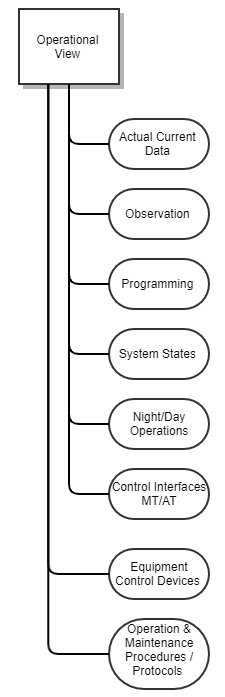
\includegraphics[scale=0.7]{access-view-operational-example}
\caption{Example of Operational Access View Tree with Root-nodes.}
\label{fig:access-view-operational-example}
\end{figure}

\begin{figure}[ht]
\centering
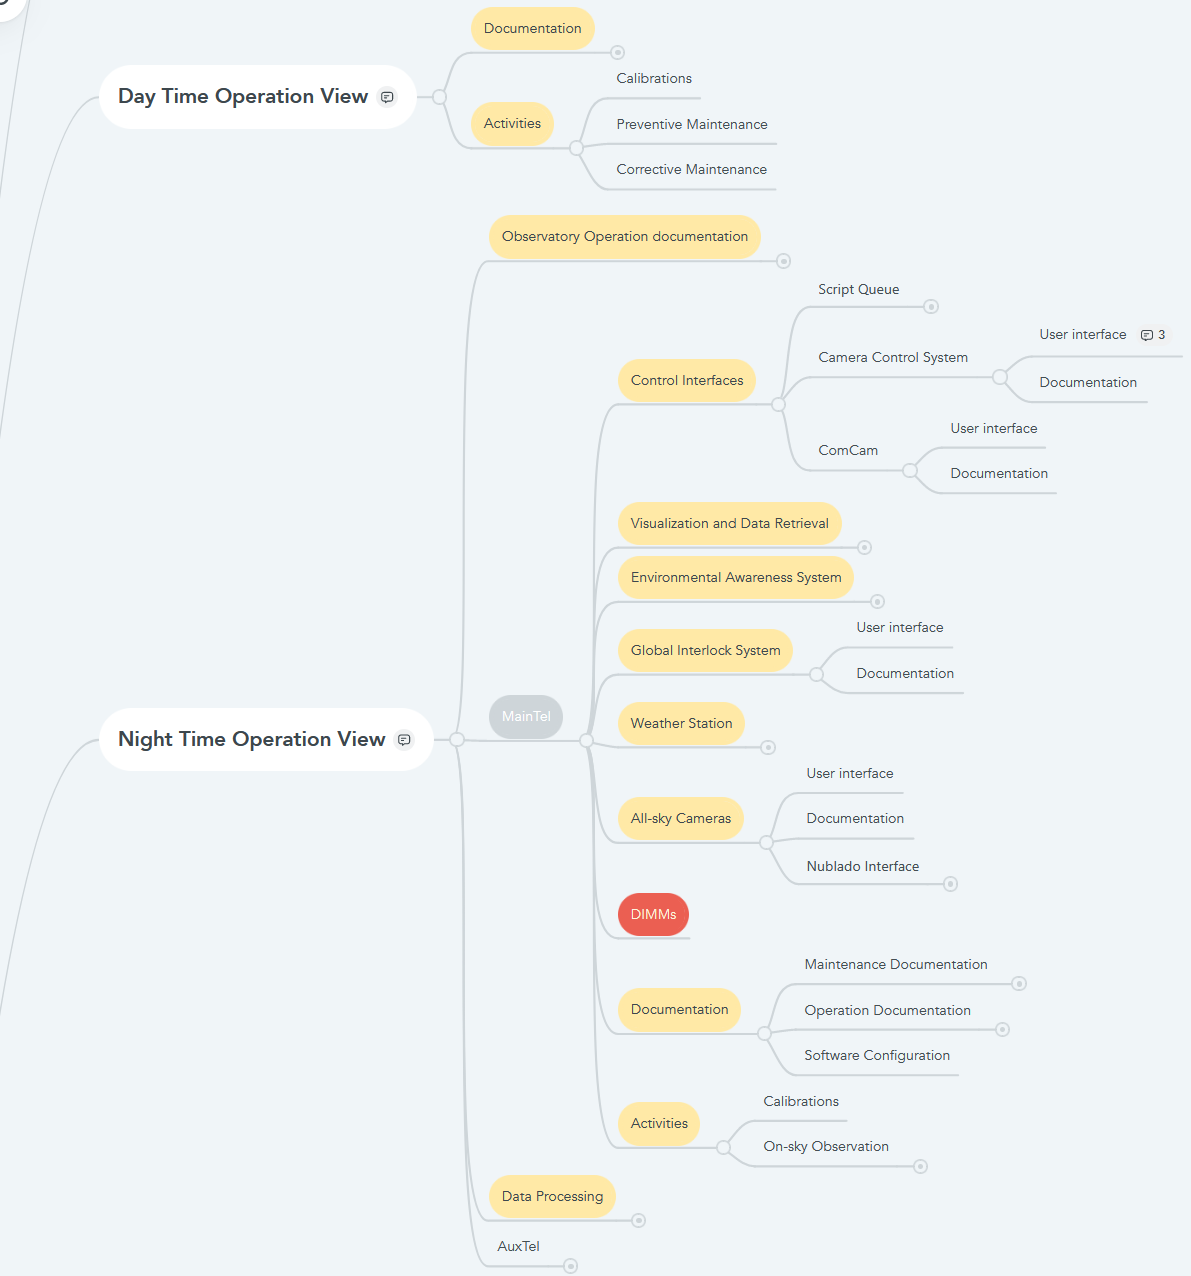
\includegraphics[width=\textwidth]{access-view-day-night-operations-example}
\caption{Example of Operational Access View Tree from Daytime and Nighttime Operations.}
\label{fig:access-view-day-night-operations-example}
\end{figure}

\subsubsection{Safety Access View}

The Safety Access View tree focuses on accessing information related directly to safety procedures and protocols that apply to the different systems.
This can help add consistency and verify requirements.
This tree would lead users to general safety procedures, specific safety procedures, emergency procedures of telescope and summit facilities (excludes emergency response).
The example provided by Figure \ref{fig:access-view-safety-example} includes safety and security aspects.
Users include safety, engineering, security, maintenance staffs and management.

\begin{figure}[ht]
\centering
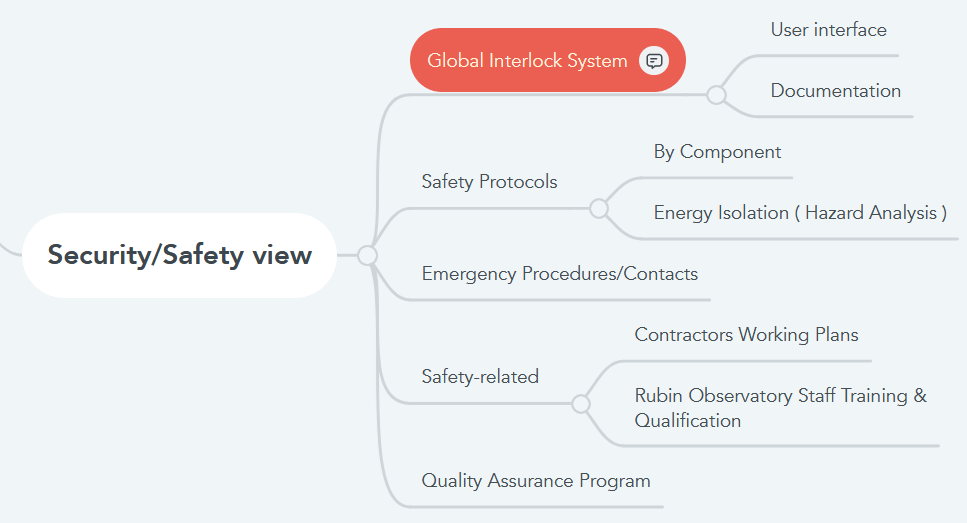
\includegraphics[width=\textwidth]{access-view-safety-example}
\caption{Example of Safety Access View Tree.}
\label{fig:access-view-safety-example}
\end{figure}

\subsubsection{Scientific Access View}

The Scientific Access View tree is for scientific platforms and interfaces that correspond or impact Rubin Observatory science objectives.
It is intended to ease access to the information by providing a clear list of the software and various databases.
An example is provided by Figure \ref{fig:access-view-scientific-example}.
Users include scientific, engineering, and observing staff and management.

\begin{figure}[ht]
\centering
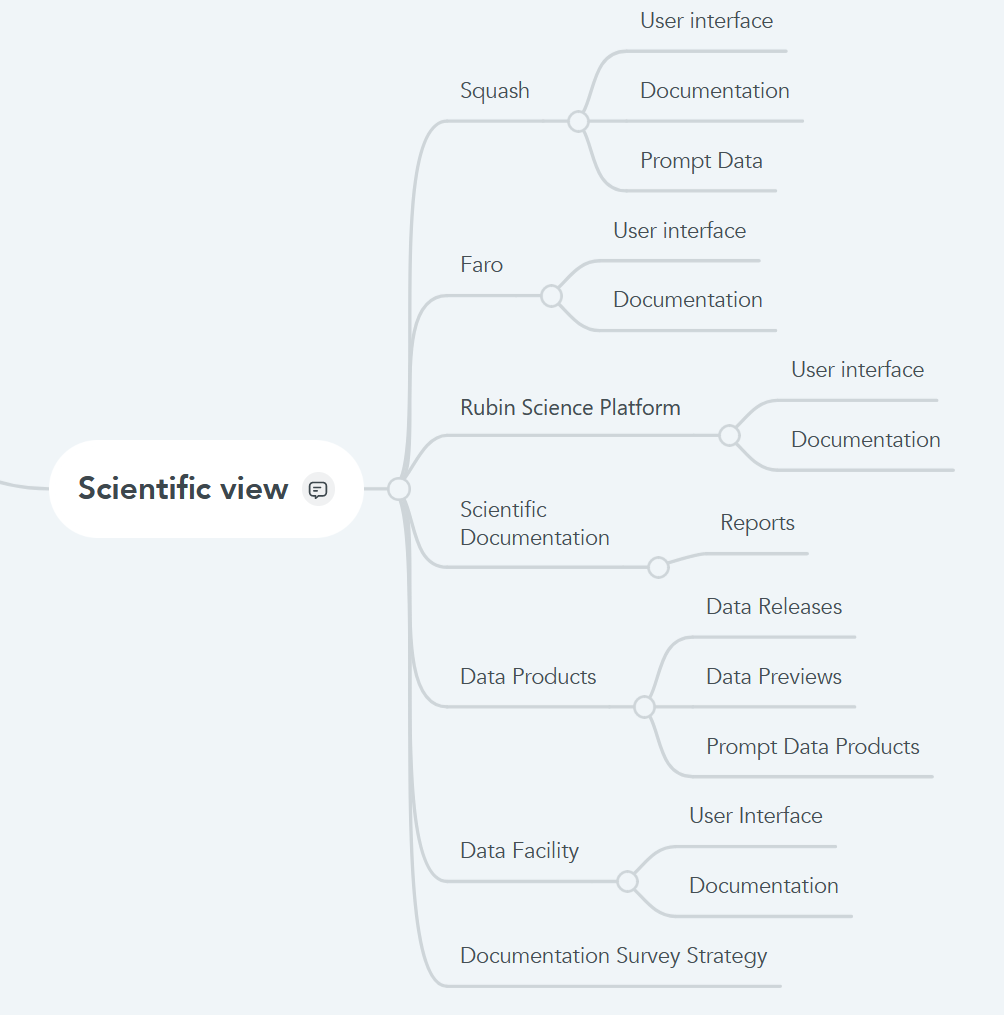
\includegraphics[width=\textwidth]{access-view-scientific-example}
\caption{Example of Scientific Access View Tree.}
\label{fig:access-view-scientific-example}
\end{figure}

\subsubsection{Engineering Access View}

The Engineering Access View tree is for accessing Rubin Observatory technical information.
In addition to the technical documentation, access interfaces and facility-related data would be needed.
An example is provided by Figure \ref{fig:access-view-engineering-example}.
Users include staff and management involved in system performance and system engineering activities.

\begin{figure}[ht]
\centering
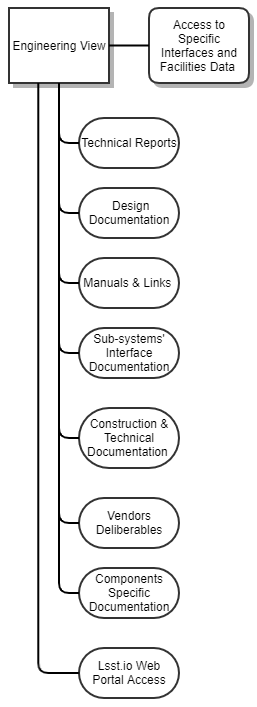
\includegraphics[scale=0.7]{access-view-engineering-example}
\caption{Example of Engineering Access View Tree.}
\label{fig:access-view-engineering-example}
\end{figure}
